\chapter{Specific Requirements} \label{specificRequirements}

\section{External Interfaces}

\begin{figure}[H]
    \centering
    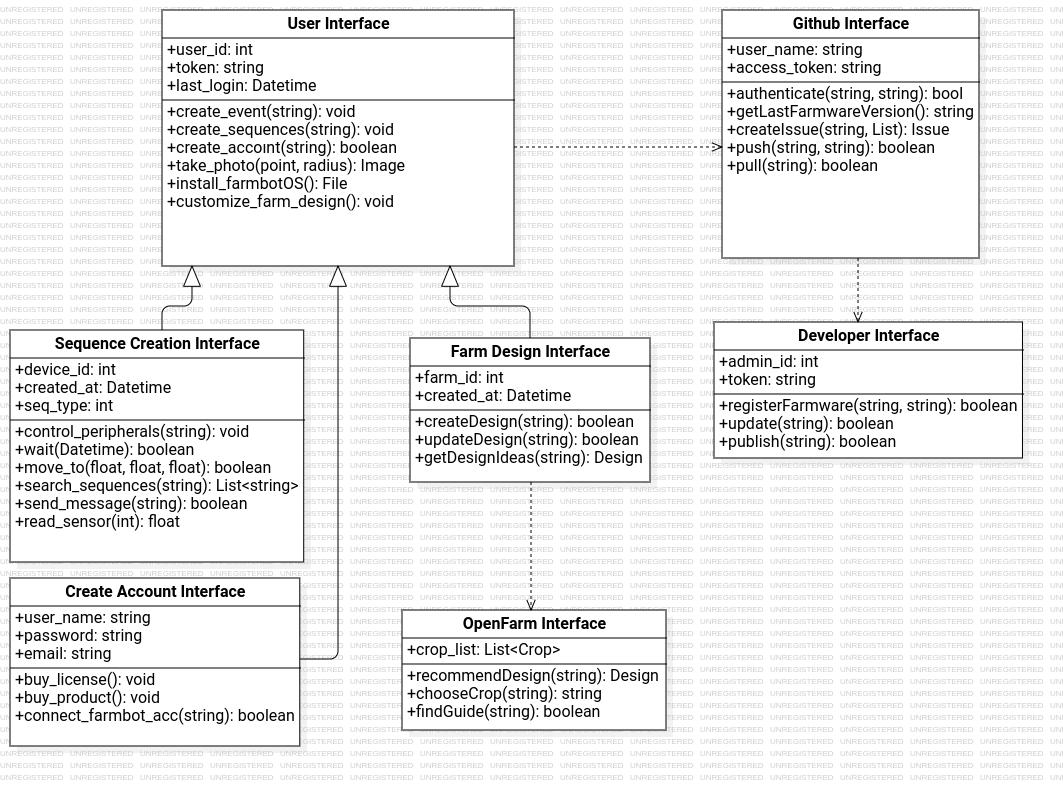
\includegraphics[width=1\textwidth]{UML Diagrams/ClassDiagram.png}
    \caption{External Interfaces Class Diagram}
    \label{fig:ExternalInterfacesClassDiagram}
\end{figure}

\begin{itemize}
  \item \textbf{User Interface}
        The user interface is the main way for the user to interact with the system. Every user has his own token and ID. Users can do some of the basic operations here, such as sequence creation, creating an account, and farm design, which can be considered as sub-interfaces of the user interface.
  \item \textbf{OpenFarm Interface}
        The OpenFarm is a free and open database for farming and gardening knowledge. The OpenFarm API is used to fetch crop data and guides for crops. The system uses OpenFarm API to get crop data and guides for crops.
  \item \textbf{GitHub Interface}
        GitHub is a code hosting platform for version control and collaboration. The system uses GitHub API to fetch the latest version of the software. It can be easily seen that the user depends on this interface to get the latest version of the software.
  \item \textbf{Developer Interface}
        The developer interface is used to interact with the system for development purposes. Developers can create new features, fix bugs, etc. Developers use this interface to contribute to the system. With further investigation, one can see that users depend on this interface to get the latest version of the software since the maintenance of the GitHub interface depends on developers.
\end{itemize}


\section{Functions}

\begin{figure}[H]
    \centering
    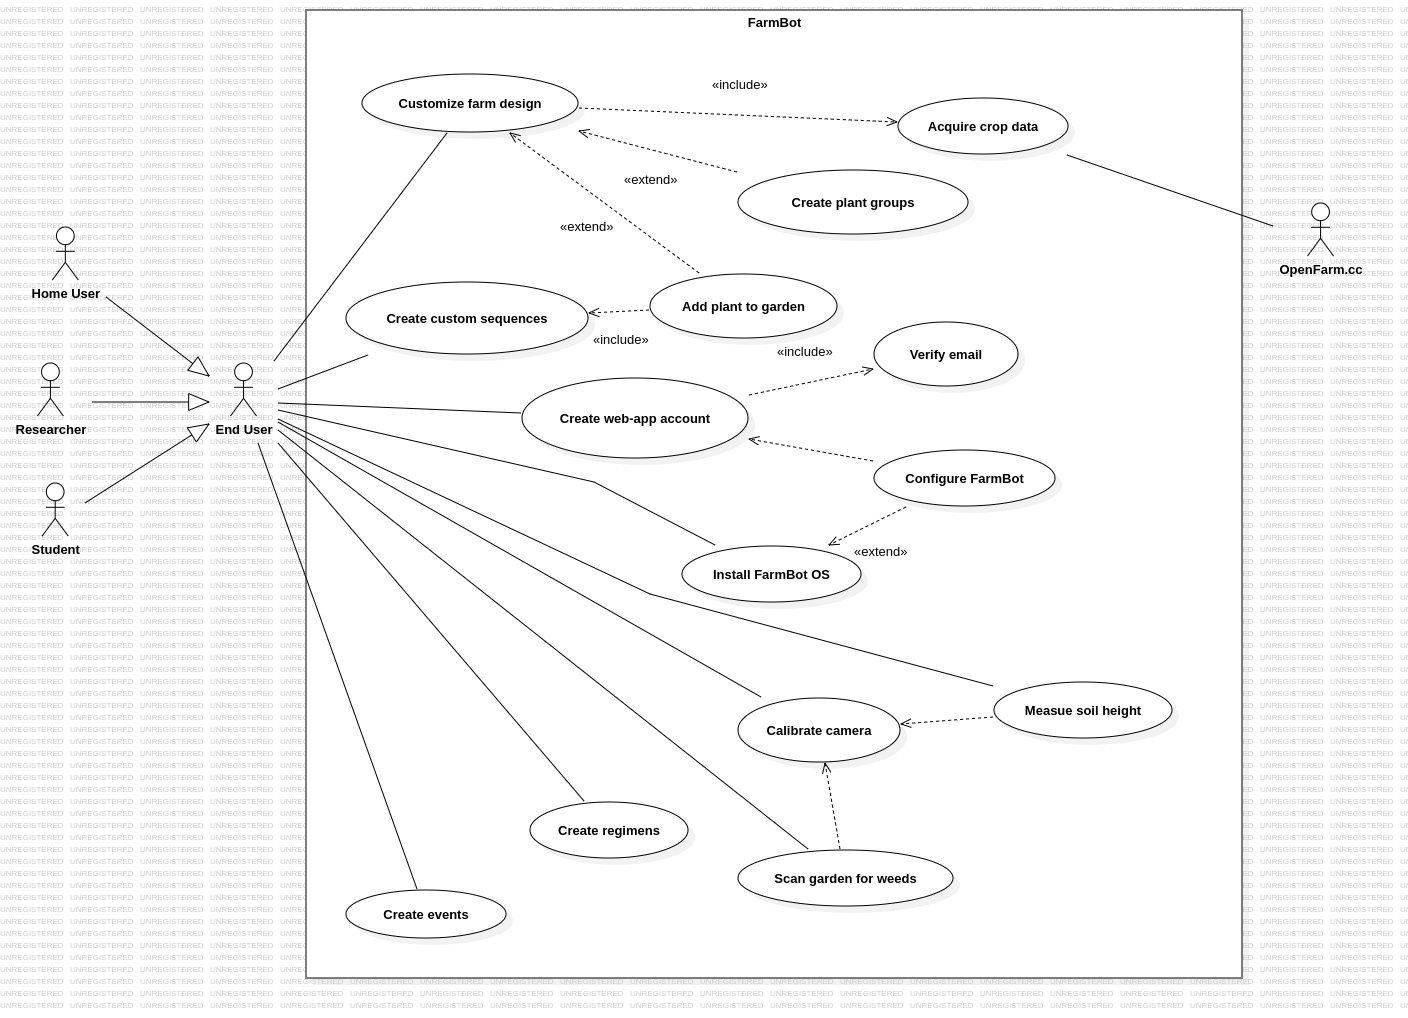
\includegraphics[width=1\textwidth]{UML Diagrams/UseCaseDiagram1.png}
    \caption{Use Case Diagram}
    \label{fig:use-case-diagram}
\end{figure}

% Please add the following required packages to your document preamble:
% \usepackage{graphicx}
\begin{table}[H]
\centering
\resizebox{\textwidth}{!}{%
\begin{tabular}{|l|l|}
\hline
\textbf{Use case name}    & Create web-app account                                                                                              \\ \hline
\textbf{Actors}           & End User                                                                                                            \\ \hline
\textbf{Description}      & The end user creates an account on the FarmBot Web App.                                                             \\ \hline
\textbf{Preconditions}    & The end user must have a valid e-mail address. The user must accept the privacy policy and terms of use.            \\ \hline
\textbf{Data}             & User credentials: e-mail, name, password                                                                            \\ \hline
\textbf{Response}         & E-mail verification link which logs user into the app                                                               \\ \hline
\textbf{Stimulus}         & The user interacts with the "CREATE AN ACCOUNT" widget.                                                             \\ \hline
\textbf{Normal Flow} &
  \begin{tabular}[c]{@{}l@{}}1. User goes to my.farm.bot\\ 2. Enters name, e-mail and password into the widget\\ 3. User checks to agree the privacy policy and terms of use\\ 4. User clicks "CREATE ACCOUNT" button\\ 5. User clicks on the verification link sent to their e-mail.\end{tabular} \\ \hline
\textbf{Alternative Flow} & -                                                                                                                   \\ \hline
\textbf{Exception Flow}   & 4. If user leaves any of the fields blank, an error pop-up appears alerting that these fields cannot be left blank. \\ \hline
\textbf{Post Conditions}  & The users account must be confirmed and user must be taken to the message center.                                   \\ \hline
\textbf{Comments}         & -                                                                                                                   \\ \hline
\end{tabular}%
}
\caption{Tabular description of create web-app account case}
\label{tab:create-account-table}
\end{table}

% Please add the following required packages to your document preamble:
% \usepackage{graphicx}
\begin{table}[H]
\centering
\resizebox{\textwidth}{!}{%
\begin{tabular}{|l|l|}
\hline
\textbf{Use case name}    & Install FarmBot OS                                                                                          \\ \hline
\textbf{Actors}           & End User                                                                                                    \\ \hline
\textbf{Description}      & The user installs FarmBot OS on the Raspberry Pi                                                            \\ \hline
\textbf{Preconditions}    & The user has a microSD card with sufficient capacity, a card reader and has downloaded Raspberry Pi Imager. \\ \hline
\textbf{Data}             & -                                                                                                           \\ \hline
\textbf{Response}         & User should see a solid red LED and a a steadily flashing green LED on the Raspberry Pi.                    \\ \hline
\textbf{Stimulus}         & User goes to os.farm.bot and clicks on the download button for respective model of FarmBot Express          \\ \hline
\textbf{Normal Flow} &
  \begin{tabular}[c]{@{}l@{}}1. User downloads the latest FarmBot OS image\\ 2. User writes the FarmBot OS onto the microSD card using Raspberry Pi Imager\\ 3. User inserts the microSD card into the Raspberry Pi\\ 4. User plugs in the power source\end{tabular} \\ \hline
\textbf{Alternative Flow} & -                                                                                                           \\ \hline
\textbf{Exception Flow} &
  \begin{tabular}[c]{@{}l@{}}2. microSD cards larger than 32GB will not work. Drag and drop or copy-paste will not work. \\ Raspberry Pi Imager must be used.\end{tabular} \\ \hline
\textbf{Post Conditions}  & LED lights should be lit, indicating that Raspberry Pi has adequate power and is busy booting up.           \\ \hline
\textbf{Comments}         & -                                                                                                           \\ \hline
\end{tabular}%
}
\caption{Tabular description of install farmbot os case}
\label{tab:install-farmbot-os}
\end{table}

% Please add the following required packages to your document preamble:
% \usepackage{graphicx}
\begin{table}[H]
\centering
\resizebox{\textwidth}{!}{%
\begin{tabular}{|l|l|}
\hline
\textbf{Use case name} & Configure FarmBot                                                                        \\ \hline
\textbf{Actors}        & End User                                                                                 \\ \hline
\textbf{Description}   & The user configures FarmBot to connect to WiFi network and web-app account               \\ \hline
\textbf{Preconditions} &
  \begin{tabular}[c]{@{}l@{}}The user must have a web app account\\ User has flashed FarmBot OS onto microSD card inserted into Raspberry Pi\\ User has an ETHERNET or WIFI connection\end{tabular} \\ \hline
\textbf{Data}          & WiFi network password and name, web-app credentials                                      \\ \hline
\textbf{Response}      & Status ticker at my.farm.bot shows that FarmBot has come online and is sending messages. \\ \hline
\textbf{Stimulus}      & Initial boot-up of FarmBot                                                               \\ \hline
\textbf{Normal Flow} &
  \begin{tabular}[c]{@{}l@{}}1. User connects to configurator\\ 2. User chooses a network type (ETHERNET or WIFI)\\ 3. User enters their web app credentials\\ 4. User submits configuration \\ 5. User makes sure that FarmBot is online\end{tabular} \\ \hline
\textbf{Alternative Flow} &
  \begin{tabular}[c]{@{}l@{}}1. If captive portal does not automatically open up, user should try navigating to setup.farm.bot or\\ 192.168.24.1 on a web browser.\\ 2. If user needs to know the network interface name or MAC address, presses the circular "i" icon.\\ 3. If user is self-hosting the web app, should go to their custom server URL\end{tabular} \\ \hline
\textbf{Exception Flow} &
  \begin{tabular}[c]{@{}l@{}}1. If user is using a smartphone, they might need to disable cellular data in order to connect to the configurator.\\ 5. If there is a problem with the configuration, the Configurator will restart within 5 minutes.\end{tabular} \\ \hline
\textbf{Post Conditions} &
  \begin{tabular}[c]{@{}l@{}}Connection between FarmBot  OS and user device is terminated.\\ Status ticker is indicating that FarmBot is online.\end{tabular} \\ \hline
\textbf{Comments}      & -                                                                                        \\ \hline
\end{tabular}%
}
\caption{Tabular description of configure FarmBot case}
\label{tab:configure-farmbot}
\end{table}

\begin{figure}[H]
    \centering
    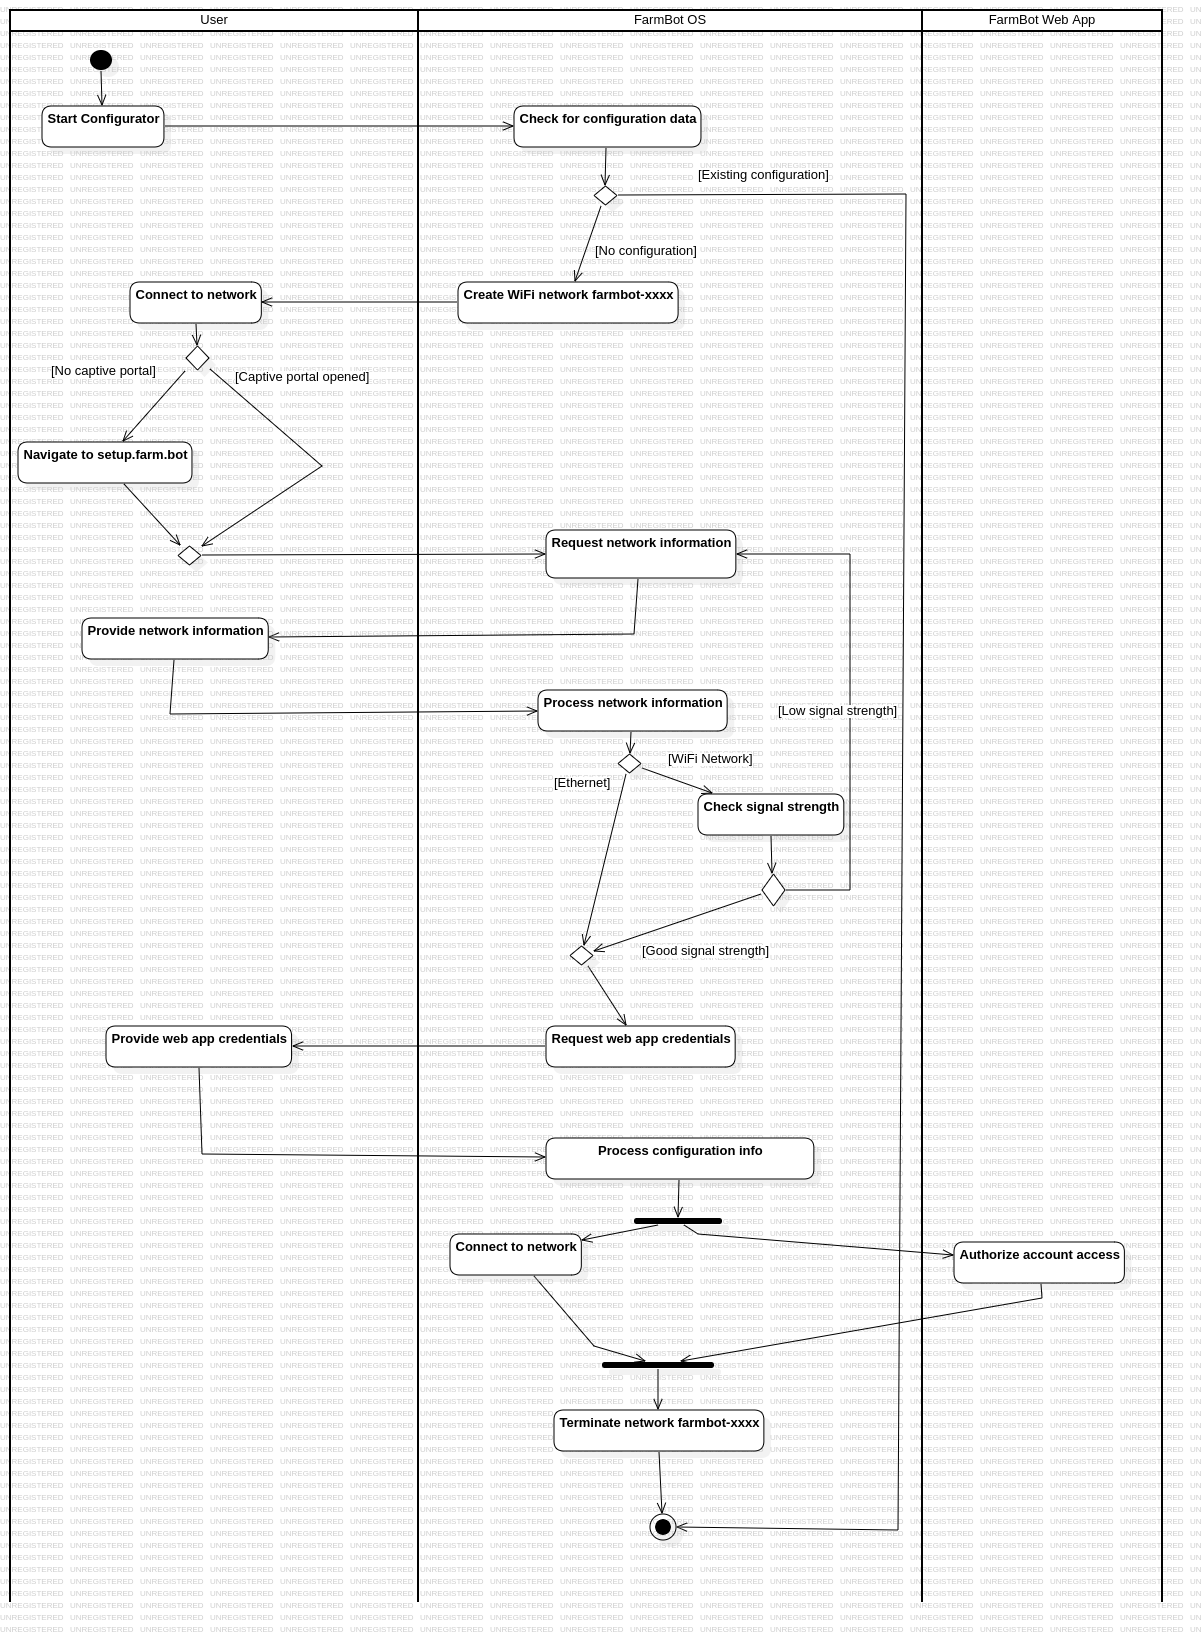
\includegraphics[width=1\textwidth]{UML Diagrams/ActivityDiagram_configurefarmbot.png}
    \caption{Activity Diagram for "Configure FarmBot" use case}
    \label{fig:configure-farmbot-activity-diagram}
\end{figure}



% Please add the following required packages to your document preamble:
% \usepackage{graphicx}
\begin{table}[H]
\centering
\resizebox{\textwidth}{!}{%
\begin{tabular}{|l|l|}
\hline
\textbf{Use case name}   & Create events                                                                                                \\ \hline
\textbf{Actors}          & End User                                                                                                       \\ \hline
\textbf{Description}     & User schedules to initiate sequences automatically                                                             \\ \hline
\textbf{Preconditions} &
  \begin{tabular}[c]{@{}l@{}}The user has a verified web-app account\\ New events must be scheduled at least one minute into the future\\ FarmBot is not performing an update\end{tabular} \\ \hline
\textbf{Data}            & Sequence or regimen data                                                                                       \\ \hline
\textbf{Response}        & The event will show up in the agenda.                                                                          \\ \hline
\textbf{Stimulus}        & User navigates to the events panel on the farm designer page and presses the "+" button for creating an event. \\ \hline
\textbf{Normal Flow} &
  \begin{tabular}[c]{@{}l@{}}1. User presses the "+" button in the events panel\\ 2. User chooses the sequence or regimen to be executed\\ 3. User provides a START date and time.\\ 4. User presses the save button to save the event.\end{tabular} \\ \hline
\textbf{Alternative Flow} &
  \begin{tabular}[c]{@{}l@{}}3. By default current date and current time + 3 minutes will be used.\\ 3. Sequence events can be set to REPEAT EVERY custom interval and UNTIL a particular stop date and time\end{tabular} \\ \hline
\textbf{Exception Flow} &
  \begin{tabular}[c]{@{}l@{}}3. New events must be scheduled at least one minute into the future, input is rejected.\\ 3. Since FarmBot performs updates at 3AM, scheduling events between 2AM and 4AM is discouraged.\end{tabular} \\ \hline
\textbf{Post Conditions} & The agenda is showing the created event and its occurrences into the future.                                    \\ \hline
\textbf{Comments}        & -                                                                                                              \\ \hline
\end{tabular}%
}
\caption{Tabular description of create events case}
\label{tab:create-events}
\end{table}

% Please add the following required packages to your document preamble:
% \usepackage{graphicx}
\begin{table}[H]
\centering
\resizebox{\textwidth}{!}{%
\begin{tabular}{|l|l|}
\hline
\textbf{Use case name} &
  Create regimens \\ \hline
\textbf{Actors} &
  End User \\ \hline
\textbf{Description} &
  \begin{tabular}[c]{@{}l@{}}User creates a regimen to easily take care of a plant throughout its entire life and allows reuse of "recipe"\\ season after season.\end{tabular} \\ \hline
\textbf{Preconditions} &
  User has created sequences to add to the regimen \\ \hline
\textbf{Data} &
  Sequence data, date and time \\ \hline
\textbf{Response} &
  The regimen will be visible on the scheduler page \\ \hline
\textbf{Stimulus} &
  User presses the "+" button on the Regimens panel \\ \hline
\textbf{Normal Flow} &
  \begin{tabular}[c]{@{}l@{}}1. User gives a descriptive name to the regimen loaded into the panel\\ 2. User presses the "SCHEDULE ITEM" button\\ 3. User selects sequence to add to the regimen.\\ 4. User picks a TIME and DAYS (relative to plant) for the sequence to run\\ 5. User presses "SAVE" button to save the regimen.\end{tabular} \\ \hline
\textbf{Alternative Flow} &
  \begin{tabular}[c]{@{}l@{}}1. User can optionally assign it a color\\ 3. User can delete falsely added sequences by clicking the trash can icon\end{tabular} \\ \hline
\textbf{Exception Flow} &
  4. Since FarmBot performs updates at 3AM, scheduling events between 2AM and 4AM is not allowed. \\ \hline
\textbf{Post Conditions} &
  The scheduler panel shows the regimen. Success pop-up is shown. \\ \hline
\textbf{Comments} &
  - \\ \hline
\end{tabular}%
}
\caption{Tabular description of create regimens case}
\label{tab:create-regimens}
\end{table}

% Please add the following required packages to your document preamble:
% \usepackage{graphicx}
\begin{table}[H]
\centering
\resizebox{\textwidth}{!}{%
\begin{tabular}{|l|l|}
\hline
\textbf{Use case name}   & Create custom sequences                                                                    \\ \hline
\textbf{Actors}          & End User                                                                                   \\ \hline
\textbf{Description}     & User combines the basic commands of FarmBot into more complex actions with multiple steps. \\ \hline
\textbf{Preconditions}   & User has a verified web-app account and has created a farm.                                \\ \hline
\textbf{Data}            & Commands, step parameters                                                                  \\ \hline
\textbf{Response}        & The green save button will turn gray and will have its text set to "SAVED".                \\ \hline
\textbf{Stimulus}        & User presses the "+" button on the Sequences panel                                         \\ \hline
\textbf{Normal Flow} &
  \begin{tabular}[c]{@{}l@{}}1. User presses the "+" button to create a new sequence\\ 2. User enters a unique name for the sequence\\ 3. User adds a command by pressing a "+" button using the command palette\\ 4. User defines step parameters\\ 5. User names each step\\ 6. User saves the sequence\end{tabular} \\ \hline
\textbf{Alternative Flow} &
  \begin{tabular}[c]{@{}l@{}}1. User can select an existing sequence to edit\\ 1. User can use the search box to find a sequence\\ 2. User can optionally assign a color to the sequence\\ 3. User can enter full-screen editor, where commands can be dragged-and-dropped.\\ 5. User can take advantage of AI to write the sequence name and description\end{tabular} \\ \hline
\textbf{Exception Flow}  & 2. If the name is not unique, it is rejected.                                              \\ \hline
\textbf{Post Conditions} & The green "SAVE" button turns gray and its text is set to "SAVED".                         \\ \hline
\textbf{Comments}        & -                                                                                          \\ \hline
\end{tabular}}

\caption{Tabular description of create custom sequences case}
\label{tab:create-custom-sequences}
\end{table}

% Please add the following required packages to your document preamble:
% \usepackage{graphicx}
\begin{table}[H]
\centering
\resizebox{\textwidth}{!}{%
\begin{tabular}{|l|l|}
\hline
\textbf{Use case name} &
  Add plant to garden \\ \hline
\textbf{Actors} &
  End User \\ \hline
\textbf{Description} &
  User adds plant to their garden \\ \hline
\textbf{Preconditions} &
  User has a verified web-app account and has completed FarmBot setup \\ \hline
\textbf{Data} &
  Crop data from OpenFarm \\ \hline
\textbf{Response} &
  The farm layout view will show the plant \\ \hline
\textbf{Stimulus} &
  User navigates to the plants panel and presses a button \\ \hline
\textbf{Normal Flow} &
  \begin{tabular}[c]{@{}l@{}}1. User presses the "+" button in the plants panel.\\ 2. User chooses a crop from panel\\ 3. User drags and drops the crop image into the map\end{tabular} \\ \hline
\textbf{Alternative Flow} &
  \begin{tabular}[c]{@{}l@{}}2. User can check out crop details\\ 3. User can click "ADD TO MAP" button and then drag the crop onto the map\end{tabular} \\ \hline
\textbf{Exception Flow} &
  \begin{tabular}[c]{@{}l@{}}3. If user wants to delete a plant, clicks on it and presses the "DELETE"\\ button on the panel that popped up\end{tabular} \\ \hline
\textbf{Post Conditions} &
  The map shows a crop icon at the desired location by the user \\ \hline
\textbf{Comments} &
  - \\ \hline
\end{tabular}%
}
\caption{Tabular description of add plant to garden case}
\label{tab:add-plant-garden}
\end{table}

% Please add the following required packages to your document preamble:
% \usepackage{graphicx}
\begin{table}[H]
\centering
\resizebox{\textwidth}{!}{%
\begin{tabular}{|l|l|}
\hline
\textbf{Use case name}    & Acquire crop data                             \\ \hline
\textbf{Actors}           & OpenFarm.cc                                   \\ \hline
\textbf{Description}      & Information about different crops are fetched \\ \hline
\textbf{Preconditions}    & For certain requests, tokens may be needed    \\ \hline
\textbf{Data}             & Garden data, crop data, guides for crops      \\ \hline
\textbf{Response}         & A JSON payload                                \\ \hline
\textbf{Stimulus}         & User chooses a crop on the plants panel       \\ \hline
\textbf{Normal Flow} &
  \begin{tabular}[c]{@{}l@{}}1. A request to the token endpoint is sent with user credentials\\ 2. Token is inserted to the request to be made\\ 3. GET/POST/PUT/DELETE request is sent with required payload\\ to the desired endpoint\\ 4. The response from the server is parsed\end{tabular} \\ \hline
\textbf{Alternative Flow} & 1. Some requests can be made without a token  \\ \hline
\textbf{Exception Flow} &
  \begin{tabular}[c]{@{}l@{}}4. The API responds with an error JSON payload in the case something went\\ wrong\end{tabular} \\ \hline
\textbf{Post Conditions}  & -                                             \\ \hline
\textbf{Comments}         & -                                             \\ \hline
\end{tabular}%
}
\caption{Tabular description of acquire crop data case}
\label{tab:acquire-crop-data}
\end{table}

\begin{figure}[H]
    \centering
    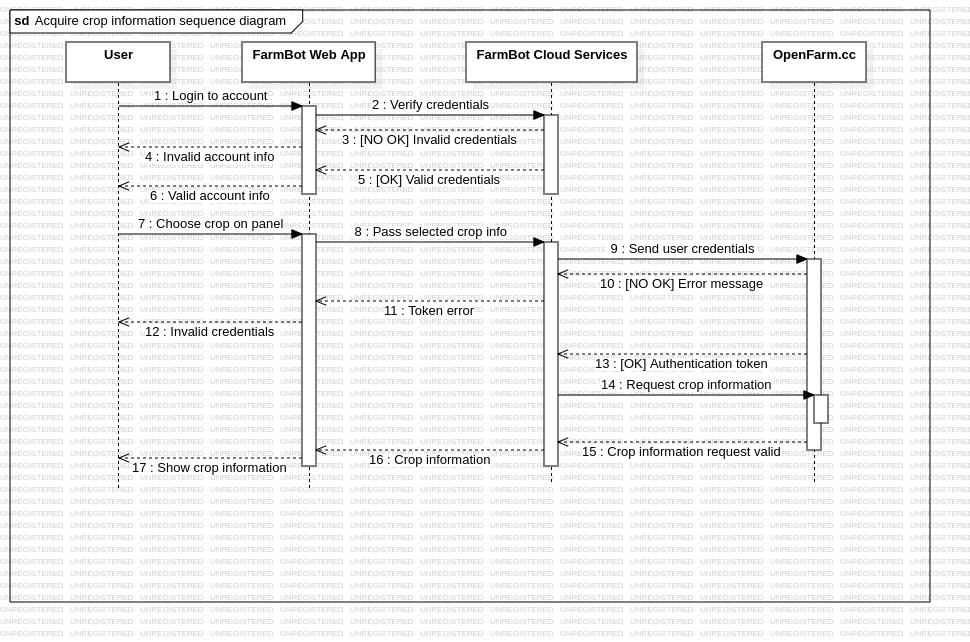
\includegraphics[width=1\textwidth]{UML Diagrams/SequenceDiagram_acquirecropinfo.png}
    \caption{Sequence Diagram for "Acquire crop data" use case}
    \label{fig:configure-farmbot-activity-diagram}
\end{figure}

% Please add the following required packages to your document preamble:
% \usepackage{graphicx}
\begin{table}[H]
\centering
\resizebox{\textwidth}{!}{%
\begin{tabular}{|l|l|}
\hline
\textbf{Use case name}    & Create plant groups                                                                    \\ \hline
\textbf{Actors}           & End User                                                                               \\ \hline
\textbf{Description}      & User groups plants, weeds or points in the garden                                      \\ \hline
\textbf{Preconditions}    & User has a verified web-app account and has completed setup                            \\ \hline
\textbf{Data}             & -                                                                                      \\ \hline
\textbf{Response}         & Group is shown on the map                                                              \\ \hline
\textbf{Stimulus}         & User navigates to the GROUPS panel and presses a button                                \\ \hline
\textbf{Normal Flow} &
  \begin{tabular}[c]{@{}l@{}}1. User opens the PLANT GROUPS, WEED GROUPS or POINT GROUPS\\ section of respective panels\\ 2. Edit group panel will be loaded with all plants, points, weeds selected\\ 3. User applies filters to narrow down selection\\ 4. User enters a name for the group\\ 5. User presses the back arrow button to save\end{tabular} \\ \hline
\textbf{Alternative Flow} & 2. User can select the multi-select mode in the farm designer and press "CREATE GROUP" \\ \hline
\textbf{Exception Flow}   & -                                                                                      \\ \hline
\textbf{Post Conditions}  & User must be able to use the groups within the sequence builder                        \\ \hline
\textbf{Comments}         & -                                                                                      \\ \hline
\end{tabular}%
}
\caption{Tabular description of create plant groups case}
\label{tab:create-plant-groups}
\end{table}

% Please add the following required packages to your document preamble:
% \usepackage{graphicx}
\begin{table}[H]
\centering
\resizebox{\textwidth}{!}{%
\begin{tabular}{|l|l|}
\hline
\textbf{Use case name}    & Customize farm design                                       \\ \hline
\textbf{Actors}           & End User                                                    \\ \hline
\textbf{Description}      & User designs the layout of their garden graphically         \\ \hline
\textbf{Preconditions}    & User has a verified web-app account and has completed setup \\ \hline
\textbf{Data}             & Crop data                                                   \\ \hline
\textbf{Response}         & Layout shown on the map                                     \\ \hline
\textbf{Stimulus}         & User navigates to the GROUPS panel and presses a button     \\ \hline
\textbf{Normal Flow} &
  \begin{tabular}[c]{@{}l@{}}1. The user sets their origin for the map\\ 2. User chooses a crops to add\\ 3. User drags and drop the crops image to the map\\ 4. User moves the crops to the desired location\end{tabular} \\ \hline
\textbf{Alternative Flow} & -                                                           \\ \hline
\textbf{Exception Flow}   & -                                                           \\ \hline
\textbf{Post Conditions}  & The plants should be at least 10mm away from each other     \\ \hline
\textbf{Comments}         & -                                                           \\ \hline
\end{tabular}%
}
\caption{Tabular description of customize farm design case}
\label{tab:customize-farm-design}
\end{table}

% Please add the following required packages to your document preamble:
% \usepackage{graphicx}
\begin{table}[H]
\centering
\resizebox{\textwidth}{!}{%
\begin{tabular}{|l|l|}
\hline
\textbf{Use case name}    & Calibrate camera                                                                   \\ \hline
\textbf{Actors}           & End User                                                                           \\ \hline
\textbf{Description}      & User calibrates camera to allow images to be rotated, positioned and calibrated    \\ \hline
\textbf{Preconditions}    & User has the camera calibration card                                               \\ \hline
\textbf{Data}             & -                                                                                  \\ \hline
\textbf{Response}         & Photos taken from the garden are shown in the farm designer with calculated values \\ \hline
\textbf{Stimulus}         & User presses the "CALIBRATE" button                                                \\ \hline
\textbf{Normal Flow} &
  \begin{tabular}[c]{@{}l@{}}1. User places the calibration card in the bed\\ 2. User moves FarmBot that the camera is positioned directly over the card\\ 3. User raises the z-axis as high as it can be raised\\ 4. User opens the photos panel\\ 5. Expands camera calibration section and presses "CALIBRATE" button\\ 6. FarmBot takes photos moving in different directions and upload them to web-app\end{tabular} \\ \hline
\textbf{Alternative Flow} & -                                                                                  \\ \hline
\textbf{Exception Flow} &
  \begin{tabular}[c]{@{}l@{}}1. If card is placed outside of the field of view, FarmBot does not detect it\\ 1. If poor lighting, user should try toggling FarmBot's LED light \\ 6. If card cannot be detected, problematic photos are uploaded. FarmBot returns to start\end{tabular} \\ \hline
\textbf{Post Conditions}  & The photos taken of the garden must line up with the grid in the farm designer.    \\ \hline
\textbf{Comments}         & -                                                                                  \\ \hline
\end{tabular}%
}
\caption{Tabular description of calibrate camera case}
\label{tab:calibrate-camera}
\end{table}

% Please add the following required packages to your document preamble:
% \usepackage{graphicx}
\begin{table}[H]
\centering
\resizebox{\textwidth}{!}{%
\begin{tabular}{|l|l|}
\hline
\textbf{Use case name}    & Scan garden for weeds                                                         \\ \hline
\textbf{Actors}           & End User                                                                      \\ \hline
\textbf{Description}      & User scans the whole garden for weeds                                         \\ \hline
\textbf{Preconditions}    & User has calibrated FarmBot's camera                                          \\ \hline
\textbf{Data}             & -                                                                             \\ \hline
\textbf{Response}         & The results are shown on the farm designer as photos                          \\ \hline
\textbf{Stimulus}         & User presses "RUN" button                                                     \\ \hline
\textbf{Normal Flow} &
  \begin{tabular}[c]{@{}l@{}}1. User creates a point grid\\ 2. User groups the points\\ 3. User creates sequences for scanning\\ 4. User presses RUN and starts scan\end{tabular} \\ \hline
\textbf{Alternative Flow} & -                                                                             \\ \hline
\textbf{Exception Flow} &
  \begin{tabular}[c]{@{}l@{}}4. After run, if the output is problematic, locations, spacing and number of points\\ in the grid may be adjusted\\ 4. Color range and other weed detection parameters may be adjusted\end{tabular} \\ \hline
\textbf{Post Conditions}  & The photos of the garden line up in the farm designer and weeds are indicated \\ \hline
\textbf{Comments}         & -                                                                             \\ \hline
\end{tabular}%
}
\caption{Tabular description of scan garden for weeds case}
\label{tab:scan-garden-for-weeds}
\end{table}

% Please add the following required packages to your document preamble:
% \usepackage{graphicx}
\begin{table}[H]
\centering
\resizebox{\textwidth}{!}{%
\begin{tabular}{|l|l|}
\hline
\textbf{Use case name}    & Measure soil height                                                             \\ \hline
\textbf{Actors}           & End User                                                                        \\ \hline
\textbf{Description}      & Using computer vision software, FarmBot detects average z-axis height of soil   \\ \hline
\textbf{Preconditions}    & User has calibrated FarmBot's camera                                            \\ \hline
\textbf{Data}             & -                                                                               \\ \hline
\textbf{Response}         & Soil height values                                                              \\ \hline
\textbf{Stimulus}         & User presses "MEASURE" button                                                   \\ \hline
\textbf{Normal Flow} &
  \begin{tabular}[c]{@{}l@{}}1. User presses the "MEASURE" button\\ 2. FarmBot takes a photos from different directions\\ 3. The photos are processed to determine the soil height\\ 4. Processed images are uploaded and soil height point is created\end{tabular} \\ \hline
\textbf{Alternative Flow} & -                                                                               \\ \hline
\textbf{Exception Flow} &
  \begin{tabular}[c]{@{}l@{}}2. If photos are problematic, user needs to recalibrate camera\\ 4. If there are outliers in the dataset, user needs to remove them.\end{tabular} \\ \hline
\textbf{Post Conditions}  & There are soil height points with measured heights across the farm designer map \\ \hline
\textbf{Comments}         & -                                                                               \\ \hline
\end{tabular}%
}
\caption{Tabular description of measure soil height case}
\label{tab:measure-soil-height}
\end{table}

\begin{figure}[H]
    \centering
    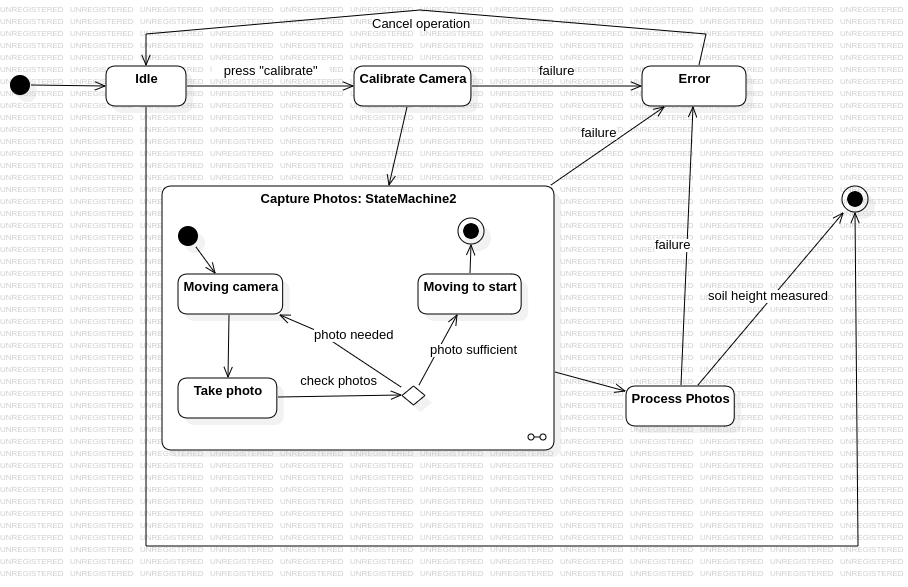
\includegraphics[width=1\textwidth]{UML Diagrams/StateDiagram_measuresoilheight.png}
    \caption{State Diagram for "Measure soil height" use case}
    \label{fig:configure-farmbot-activity-diagram}
\end{figure}

\section{Logical Database Requirements }

\begin{figure}[H]
    \centering
    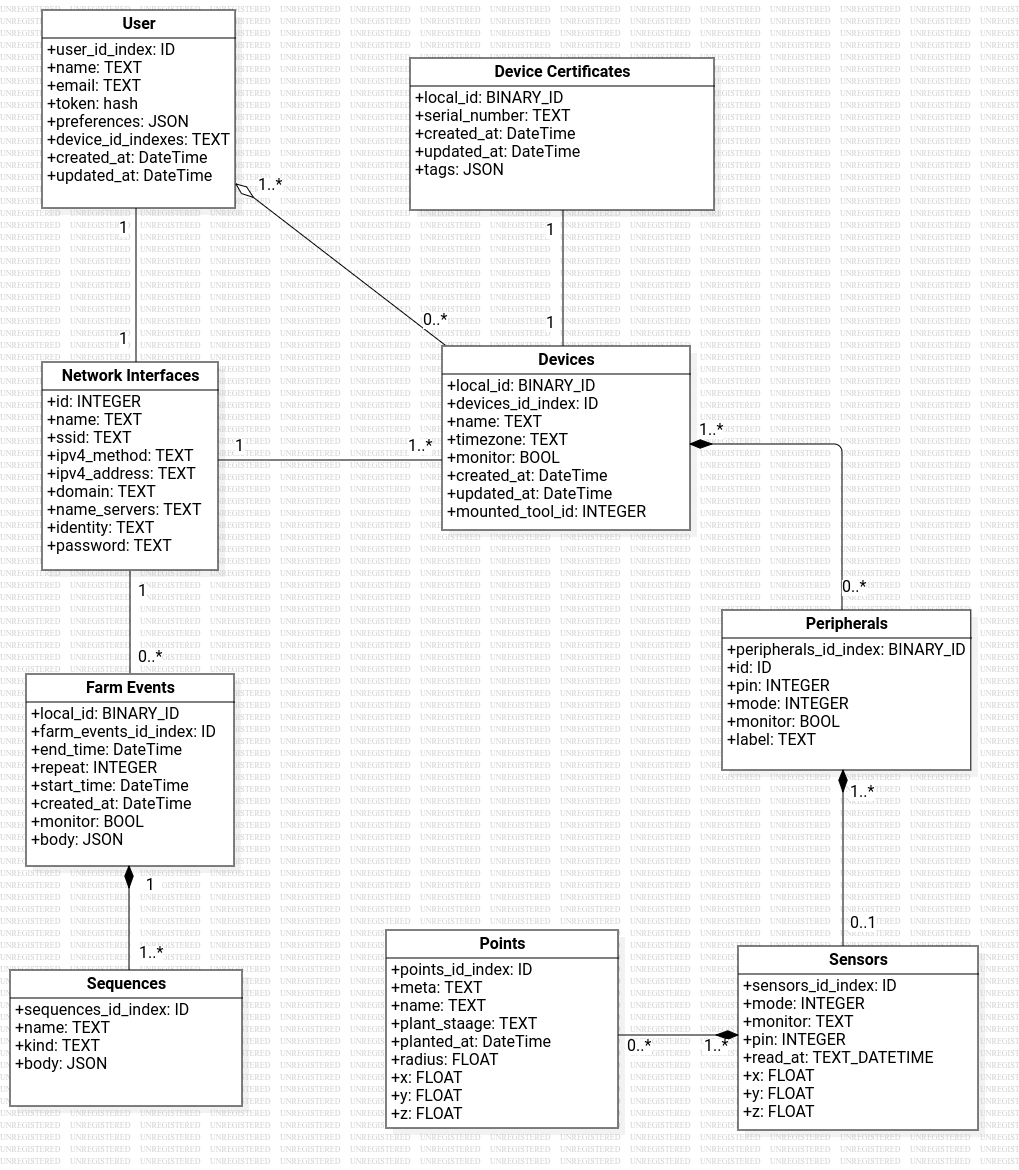
\includegraphics[width=1\textwidth]{UML Diagrams/DBDiagram.png}
    \caption{Logical Database Requirements Class Diagram}
    \label{fig:LogicalDatabaseERDiagram}
\end{figure}

The logical database requirements diagram can be seen in Figure \ref{fig:LogicalDatabaseERDiagram}. The dataflow diagram shows the relationships between the different entities in the database.
\begin{enumerate}
  \item \textbf{User} - The user entity stores the user's information, such as their name, email, password, and role. The user can have multiple farm devices. The user can create multiple farm events using the network interface of the web app.
  \item \textbf{Devices} - The farm device entity stores the device's information, such as its name, device type, and status. The device can access multiple farm events using the web app network interface. The farm device can have multiple farm sequences, too. Furthermore, the device can have multiple peripherals with external sensors. Finally, every device has its own device certification.
  \item \textbf{Network Interface} - The network interface entity stores the network interface's information, such as its name, type, and status. The network interface basically a bridge between the device and the web app. Here the protocols, IP addresses, and ports are stored.
  \item \textbf{Farm Events} - The farm event entity stores the event's information, such as its name, type, and status. The farm event can have multiple farm sequences. It is a user-created event that can be scheduled to run at a specific time.
  \item \textbf{Sequences} - The farm sequence entity stores the sequence's information, such as its name, type, and status. The farm sequence can have multiple farm commands.
\end{enumerate}

\section{Design Constraints}

FarmBot software is an open-source development project. Therefore clear guidelines for contribution, documentation and version control is needed. The software is licensed with the MIT license approved by the Open Source Initiative and a free license by Free Software Foundation. The documentation is licensed under the CCO Public Domain Dedication.

FarmBot collects user data such as their web-app credentials, photos from their gardens, their plant schedules. The software comply with the data privacy regulations GDPR (General Data Protection Regulation), CCPA (California Consumer Privacy Act).

FarmBot software has certifications to prove that it is compliant with user safety regulations. The Raspberry Pi comply with RoHS (Restriction of Hazardous Substances), FCC (Federal Communications Comission) certifications. Farmduino is compliant with CE certification meaning that the product conforms European health, safety, environmental protection standards and is compliant with RoHS certification.

\section{System Quality Attributes}

\subsection{Usability Requirements}
\begin{itemize}
    \item The system should be easy to set up, operate and maintain in order to be accessible to people with minimal technical knowledge.
    \item The software should be intuitive for learning basic gardening principles and experimentation for a good learning experience for students. Data visualizations and analysis components must be easy to understand and use since student's knowledge is minimal.
    \item The system should allow for precise control over planting parameters, data collection and export of data for research to be done.
    \item The interfaces should be accessible, working well with screen readers and feature adjustable font sizes to accommodate different users needs.
    \item The system should allow for automation of repetitive tasks so that researchers can focus on more important tasks.
    \item The user interface should be visually appealing, user-friendly, and must provide clear feedback on system status and actions.
    \item The system should offer a sense of accomplishment and provide a fun farming experience for home users to take part in as a family.
\end{itemize}

\subsection{Performance Requirements}
\begin{itemize}
    \item FarmBot supports two user interfaces (terminals):
    \begin{enumerate}
        \item FarmBot Web App (Browser)
        \item FarmBot Configurator (Raspberry Pi)
    \end{enumerate}
    \item Sensor data, camera data must be transferred between web-app and device in real-time. The messaging queue must process a million MQQT messages per second providing miliseconds-level of latency. 
\end{itemize}

\subsection{Reliability}
\begin{itemize}
    \item Transfer of sensor, camera data between FarmBot device and web-app shall be accurate, without loss and real-time.
\end{itemize}

\subsection{Availability}
\begin{itemize}
    \item FarmBot should be available to execute custom sequences, events, and/or regimens 91.67 percent of the day. It performs updates between 3AM - 5AM.
    \item If the device attempts to connect to the message broker more than 20 times in a 10 minute period, it will be temporarily blocked for 10 minutes.
\end{itemize}

\subsection{Security}
\begin{itemize}
    \item FarmBot device logs and web-app logs must be maintained to track user activity, system events and potential security breaches.
    \item Communication between critical software componenets are restricted via the use of tokens while using the APIs.
    \item Data validation and error checking mechanisms are implemented to ensure accuracy of user data and inputs.
\end{itemize}

\subsection{Maintainability}
\begin{itemize}
    \item Modular design and well-defined interfaces between different components are crucial for independent development, testing and debugging.
    \item A clear and concise documentation is needed for future maintenance.
    \item A version control system must be utilized for tracking changes and rolling back if necessary.
    \item Unit tests and integration tests must be created to realize and fix problems efficiently.
\end{itemize}

\subsection{Portability}
\begin{itemize}
    \item The web-app must allow using modern web standards to be compatible with different devices and browsers.
\end{itemize}

\section{Supporting Information}

FarmBot is an open-source and scalable automated precision farming machine. FarmBot automates repetitive tasks such as planting seeds, watering, and applying nutrients. It allows precise control over various planting parameters like seed spacing, watering schedules. It provides a data-driven approach to farming using various sensor data and crop information from OpenFarm. OpenFarm is a free and open database for farming and gardening knowledge. FarmBot can be a valuable tool for students and educators interested in learning about different STEM objectives. Robotics, agriculture and automation are some of them. 


